\section{Введение}
Современные объектно ориентированные языки программирования, такие как Java, предоставляют удобные механизмы для написания программ. Обычно приложения представляют собой огромное число различных объектов. 
\par
Однако такая декомпозиция программ может приводить к негативному влиянию на производительность. Огромное число мелких объектов приводит к фрагментации памяти, плохой локальности процессорного кеша, а также к увеличению числа чтений указателей из памяти. Эти факторы неизбежно приводят к ухудшению производительности Java приложения.
\par
В этой работе предлагается способ, как можно уменьшить негативное влияние вышеперечисленных недостатков введением в язык Java новой структуры данных, названной flattened array или FlatArray. Она представляет собой последовательность объектов, расположенных в одном линейном участке памяти. 
Для Java программиста flattened массив имеет интерфейс обычного Java класса.
\par
Flattened array может быть применен для реализации многих других структур данных и алгоритмов, зависящих от скорости доступа к памяти. В частности, в данной работе была реализована альтернативная версия хеш-таблицы, которая в некоторых случаях показала лучшую производительность операции поиска.
\par
На рисунке \ref{ref-graph} изображен граф объектов, который может быть частью объектно-ориентированного приложения.
\begin{figure}[h]
	\caption{Массив объектов класса Point}\label{ref-graph}
	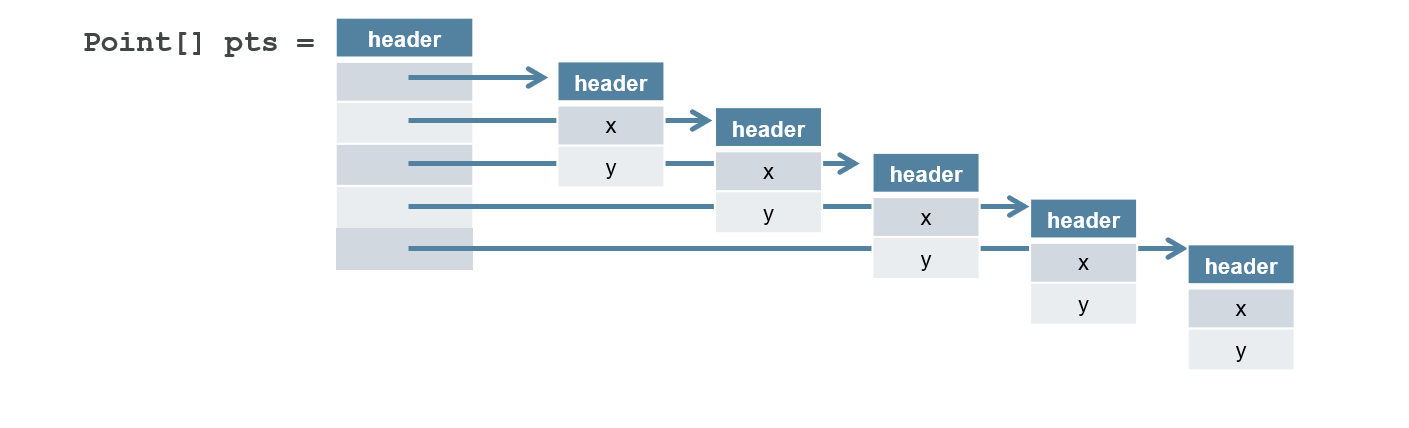
\includegraphics[width=0.95\linewidth]{image/reference.png}
\end{figure}
Класс Point содержит в себе два поля x, y типа int. Как описывалось ранее, Java работает с 
такого рода объектами как со ссылками. Потому массив "pts" содержит в себе указатели. В таком случае при доступе к полю "x" элемента i требуется дополнительное разыменования указателя, и только потом поступаемся по поля x.
\begin{lstlisting}
Point value = pts[i].x;
\end{lstlisting}
Однако в реальности мы имеем дополнительные издержки, связанные с исполнением load барьера и проверкой прочитанного значения на null:
\begin{lstlisting}
	Point* tmp = &pts[i];
	Point actual_value = load-barrier(tmp);
	if (actual_value == null) {
		throw new NullPointerException();
	}
\end{lstlisting}
В итоге это приводит к довольно дорогостоящему доступу к элементу массива. Было бы полезно избавиться от дополнительных накладных расходов на доступ к полю. Одним из возможных способов является расположение всего массива в виде линейного участка памяти, как указано на рисунке \ref{values-graph}.

\begin{figure}[h]
	\caption{Массив значений}\label{values-graph}
	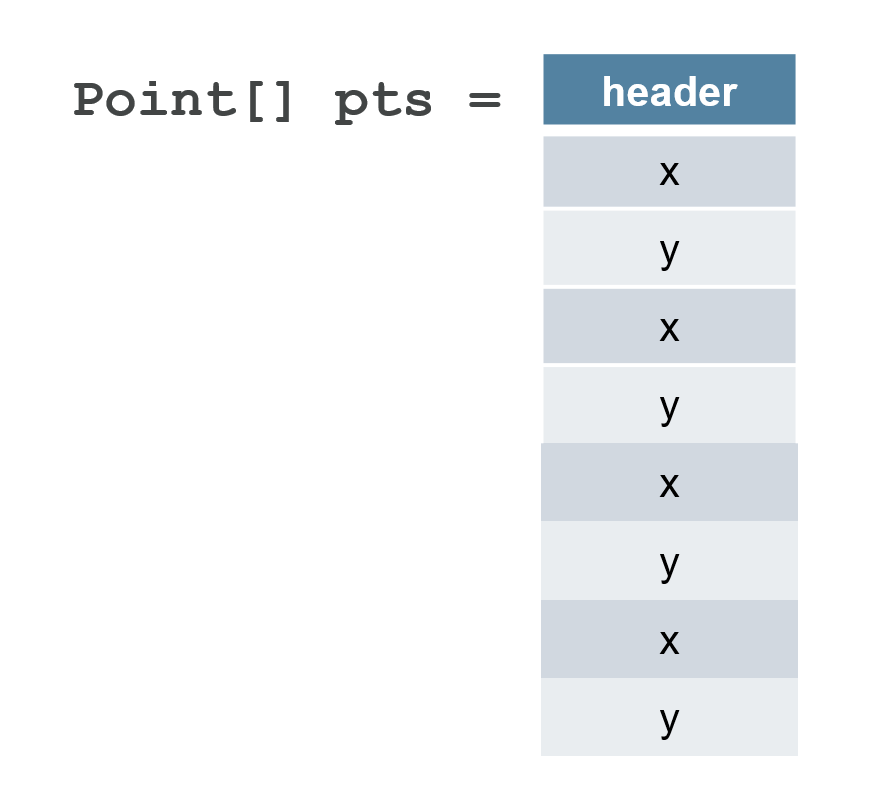
\includegraphics[width=0.65\linewidth]{image/flattened-points.png}
\end{figure}
По сравнению с предыдущей раскладкой объектов, у последней есть ряд преимуществ:
\begin{itemize}
	\item Улучшается локальность процессорного кеша. Поскольку объекты находятся рядом, а не разбросаны по всей куче, при чтении одного элемента в линейку кеша могут быть записаны соседние элементы. Это потенциально увеличивает производительность последовательного доступа к элементам массива.
	\item Удаляются load барьер и проверка на null. Адрес конкретного поля i-того элемента могут быть вычислен с помощью простой арифметики. Во многих случаях это обходится дешевле чтения ссылки из памяти. И поскольку виртуальная машина подразумевает, что в таком массиве не бывает указателей, равных null, проверки на null исчезают.
	\item Последовательный доступ к элементам может быть автоматически векторизован компилятором
\end{itemize}
К сожалению, на данный момент JVM и язык Java не поддерживают возможность создания такого рода структуры данных. Данная работа посвящена ее разработке. Для этого были поставлены следующие задачи: 
\begin{enumerate}
	\item Изучить похожие работы
	\item Реализовать данную структуру данных. Она подразумевает разработку интерфейса для Java программиста, поддержку на уровне среды исполнения
	\item Измерить производительность и проанализировать результаты
	\item Изучить применимость данной структуры данных для реализации других. Так же провести тестирование производительности.
\end{enumerate}
Данная работа проводилась на базе виртуальной машины Zing. Главными отличиями этой JVM от OpenJDK является замена С2 компилятором Falcon, базирующемся на LLVM, и применением конкурентного сборщика мусора С4\cite{C4collector}. Ее более подробное описание можно найти в секции \ref{view}.
\clearpage
